\documentclass{article}
\usepackage{graphicx}
\usepackage[margin=2cm]{geometry}

\title{\Huge \textbf{AppleStocks}\\\vspace{0.2em} \Large A Simple Application for Apple Stock Quotes Monitoring}
\author{
    Henrique Romão \\ 
    \textit{up202108067@up.pt} 
    \and 
    Mariana Bessa \\ 
    \textit{up202107946@up.pt}
}

\begin{document}

\maketitle

\begin{abstract}
    To be written at the end.
    % [TO-DO]
\end{abstract}

\section{Introduction}
This application was developed to provide users with a simple and intuitive way to view Apple stock quotes for a selected recent period. 
Users can customize their experience by choosing the time interval (in days or hours) and the duration of the interval, which can range from 2 to 10.

\section{Use Cases}
The application supports the following use cases:
\begin{itemize}
    \item Choose View Options - where the user selects a time interval (hourly or daily) and a range (2–10).
    \item Get Stock Information - where the the application connects with the Web API.
    \item See Stocks - when the user pushes the "Submit" button and sees the Plot Activity.
\end{itemize}

\begin{figure}[h!]
    \centering
    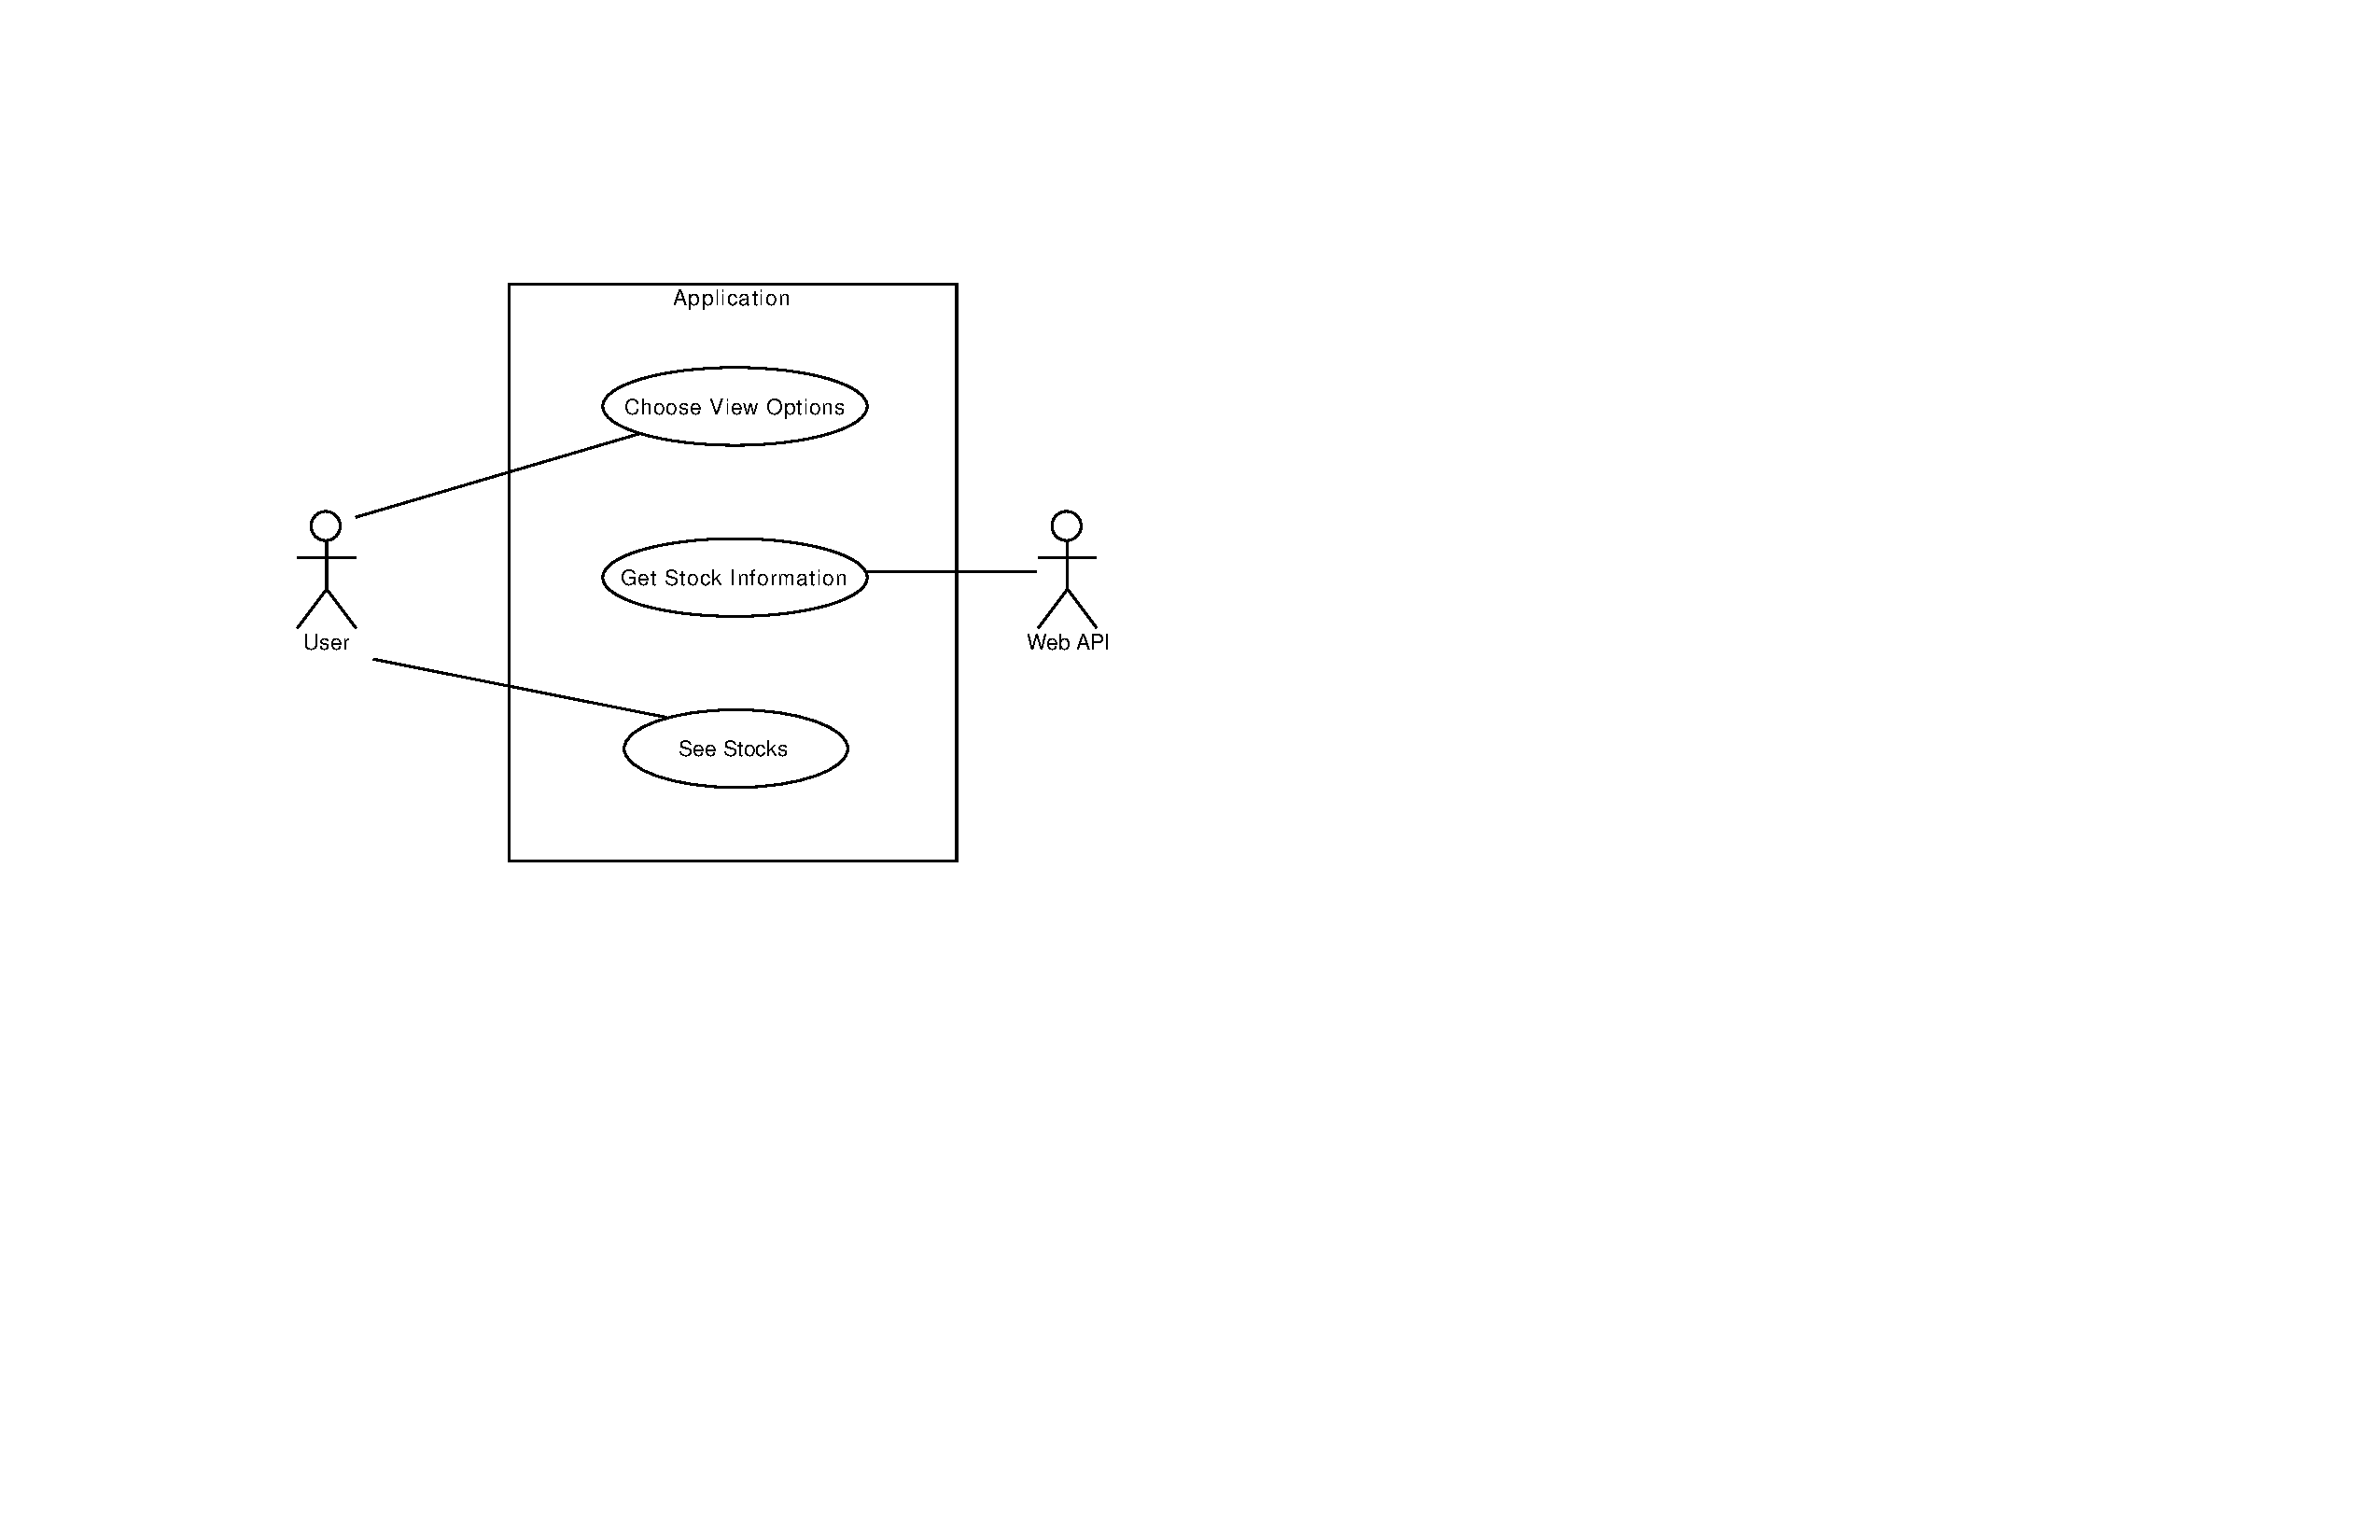
\includegraphics[width=0.6\linewidth]{Use Cases.pdf}
    \caption{Use Cases Diagram.}
    \label{fig:UseCases}
\end{figure}

\section{Architecture}
This application was developed to offer users a straightforward and intuitive way to view Apple stock quotes over a chosen recent period. Users can adjust their experience by selecting the type of time interval (in days or hours) and the duration of the interval, which can range from 2 to 10 intervals.

To enhance usability, the application was divided into two activities: the \textbf{Main Activity}, where the user configures their preferences, and the \textbf{Plot Activity}, where the results are displayed.

\subsection{Main Activity}
The Main Activity features an action bar displaying the name and logo of the app. 
It also includes two \textbf{Spinner} objects: one for selecting the type of interval (hours or days) and another for specifying the interval range. 
These spinners are initialized in the Main Activity code using the \texttt{new ArrayAdapter<>()} method, with \texttt{setDropDownViewResource} used to define their layout.

Both spinners have default values: "H" (hours) for the type of interval and "2" for the range. 
This means that, unless changed by the user, the stock quotes for the last two hours will be displayed by default.

A button is provided to allow the user to proceed. Its listener is implemented within the Main Activity. The \texttt{onClick()} method creates an \textbf{Intent} to open the Plot Activity, passing the user's spinner selections (as a string and an integer) to the new activity.

\subsection{Plot Activity}

\section{Interface}
The application has a black background with purple accents, as these darker colors are more associated with the stock market. The theme used was \texttt{Theme.AppCompat.Light.DarkActionBar}.

\subsection{Main Activity}
Upon opening the application, the user is welcomed by an action bar and two text views that display a greeting and provide instructions on how to use the app. Below these, additional text views explain the purpose of each spinner.

The layout is organized within a \textbf{LinearLayout} to arrange the text views, spinners, and the submit button vertically. The design ensures that the interface adapts well to both vertical and horizontal screen orientations, maintaining a consistent and user-friendly layout.

When the "Submit" button is pressed, the application launches the Plot Activity using the \texttt{startActivity()} method, passing the user's selected options as extras.

The layout of the spinner items and drop-down items was customly made in the \texttt{/layout/spinner\_dropdown\_item.xml} and \texttt{/layout/spinner\_item.xml} files. 
The values displayed in the Spinner views were defined in the \texttt{strings.xml} file located in \texttt{src/main/res/values/}. The button was adapted to one with rounder corners through the 

% [COMMENT] [BESSA] HENRIQEU HELP ESTA A SAIR DAS MARGENS

\subsection{Plot Activity}

\section{User Experience}
The application prioritizes simplicity and ease of use. The Main Activity's clean layout and clear instructions ensure users can quickly configure their preferences, while the Plot Activity delivers an engaging and informative visual representation of stock data.

\end{document}
